\section{The System}

% High-level architecture

\begin{figure}
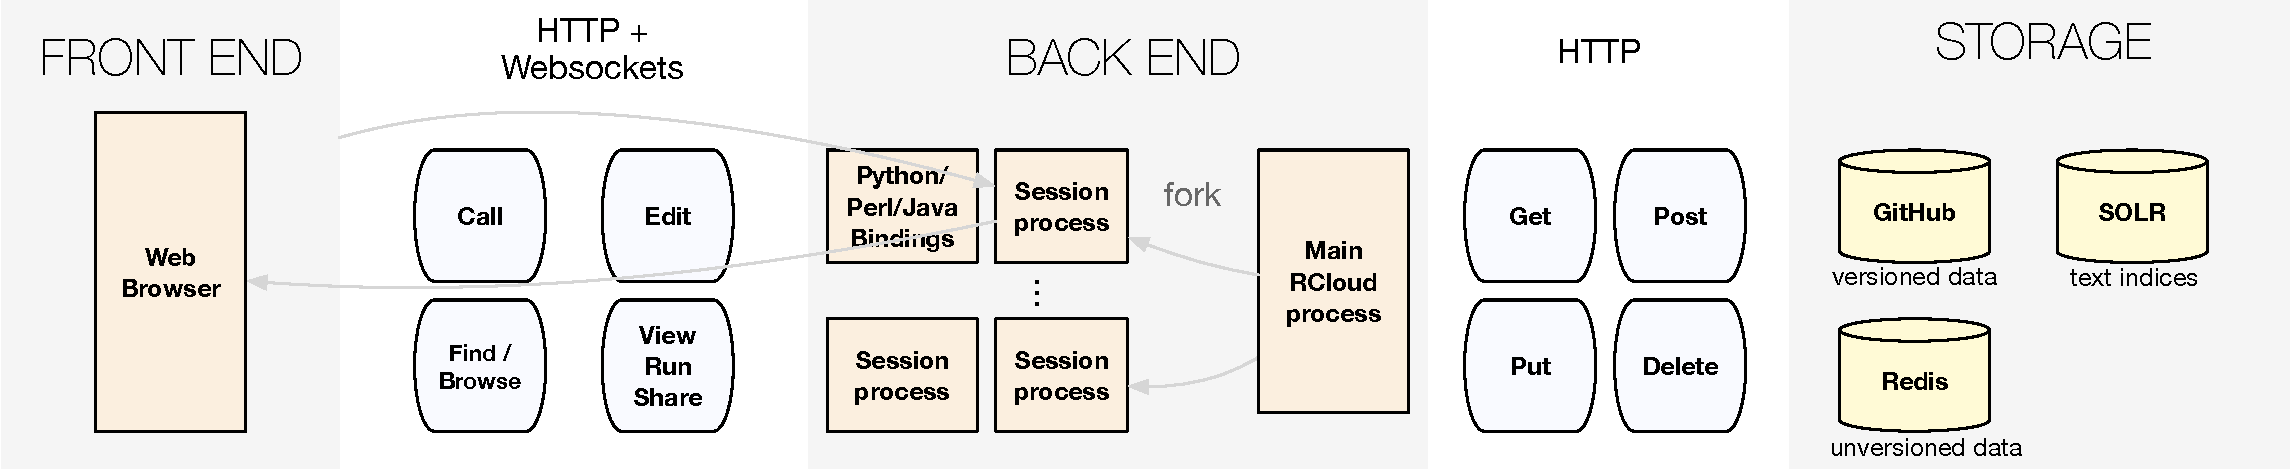
\includegraphics[width=\linewidth]{fig/system/system.pdf}
\caption{\label{fig:system}A diagram of RCloud's architecture. Dashed
  lines represent features which not yet implemented.}
\end{figure}

The internal computing infrastructure of organizations has changed
radically in the last fifteen years or so. Much of the move toward the
``cloud'' brought with it an ecosystem of processes distributed over a
network (many times virtually defined) that communicate over a
high-level protocol of some sort. Messages are typically exchanged
over HTTP. HTTP is attractive because web browsers and servers are
ubiquituous and available in essentially all pieces hardware today,
from tiny sensors in sensor networks to handheld devices to laptops to
rack-mounted servers.

As a result, in our view HTTP has become the lingua franca of IPC in
an intranet. One of the design goals for RCloud was to provide an
attractive environment for creators of data-analysis scripts, but at
the same time to create a system that behaves as a first-class citizen
in the ecosystem of computer services and networks with an
organization.

%% Design for cloud-friendly? This goes back to the point in the
%% introduction about playing nice with the rest of the ecosystem.

\subsection{System Design}

We designed RCloud around the front-facing API, which has roughly one
entry point for each requirement.

Edit

View/Run/Share

Call

Browse/Search. ``More like this'', and a custom webpage solely for browsing.

\subsection{Notebooks\label{sec:notebooks}}

Notebooks as Github gists. 
%
We needed version control over a directory, gist provides that,
wrapped over an HTTP interface.
%
Mainly a tactical decision to save time.
%
Nevertheless, availability of notebook data as (barely) plain text had good side
effects, like ease to build search. 
%
Expect same with suggest.

\subsection{Reputation and Interest: starring\label{sec:starring}}

In RCloud, reputation and interest are a relationship between
\emph{notebooks} and \emph{users}, rather than a relationship between
user pairs. We decided on this approach because we expect typical
RCloud deployments to have relatively few users, but each user to have
 written relatively many notebooks.
In this case, assigning interest to users would not provide
``high-resolution'' data.

Explicit signaling of interest: starring.

Implicit signaling of interest: click-through count and execution
count.

These will be ingredients for the recommendation system.

\subsection{Deployment of notebooks\label{sec:deployment}}

Notebooks as versioned subroutines, web services.

Notebooks by default are visible by the entire organization: there
exists a URL for every notebook in RCloud. This is deliberate. As
pointed out by Wattenberg and Kriss~\cite{Wattenberg:2011:DFS}, broad
access to analysis outputs (in their case, in the form of NameVoyager)
increases long-term engagement partly by the crossreferences in the
web. Our main RCloud deployment is only visible inside an intranet,
but we have nevertheless found anecdotal support for this theory by
noticing links to RCloud notebooks in internal discussion fora and
mailing lists.

\subsection{Technologies: R, Python, HTML5, interactive notebooks, etc.}

How do we do things that are not trivial to do with IPython (for example)

dcplot. two-way communication between between backend session and
frontend session.
